\subsection{Legge della Probabilità Totale per PDF e Medie}

In modo analogo al caso discreto, presa una qualunque partizione $\{E_m\}_{m=1}^M$ di $\Omega$, allora:

\begin{equation}
f_X(x) = \sum_{m=1}^{M} f_{X|E_m}(x)\mathbb{P}(E_m) \iff F_X(x) = \sum_{m=1}^{M} F_{X|E_m}(x)\mathbb{P}(E_m)
\end{equation}

Naturalmente, questo implica che per le medie valga un'analoga relazione (vedi slide 57):

\begin{equation}
\mathbb{E}[X] = \sum_{m=1}^{M} \mathbb{E}[X|E_m]\mathbb{P}(E_m) = \sum_{m=1}^{M} \mathbb{P}(E_m) \int_{\mathbb{R}} x f_{X|E_m}(x) dx
\end{equation}

\subsubsection*{Dimostrazione}

Il teorema della probabilità totale vale per la CDF, che in forma estesa si scrive nel seguente modo:

\begin{equation}
\mathbb{P}(X \le x) = \sum_m \mathbb{P}(E_m) \mathbb{P}(X \le x | E_m) = \sum_m \mathbb{P}(E_m) F_{X|E_m}(x)
\end{equation}

Per definizione di valore atteso e per il teorema della probabilità totale applicato alla PDF abbiamo che:

\begin{equation}
\mathbb{E}[X] = \int_{\mathbb{R}} x f_X(x) dx = \int_{\mathbb{R}} x \left[ \sum_m \mathbb{P}(E_m) f_{X|E_m}(x) \right] dx
\end{equation}

L'integrale di una somma è uguale alla somma degli integrali; inoltre, $\mathbb{P}(E_m)$ non dipende da $x$, quindi:

\begin{equation}
\sum_m \mathbb{P}(E_m) \underbrace{\int_{\mathbb{R}} x f_{X|E_m}(x) dx}_{\mathbb{E}[X|E_m]} = \sum_m \mathbb{P}(E_m) \mathbb{E}[X|E_m] = \mathbb{E}[X]
\end{equation}


\section{Funzioni di Variabili Aleatorie Continue}

Quest'argomento riproduce - come problematica - quello già affrontato nel caso di variabili discrete (vedi slide 58 e seguenti).

\begin{itemize}
    \item Si assuma che $X = X(\omega)$ sia una variabile aleatoria continua con alfabeto $\mathcal{X}$, PDF $f_X(x)$ e CDF $F_X(x)$.
    \item Sia $g(\cdot)$ una funzione il cui insieme di definizione includa i punti di $\mathcal{X}$ - a meno di un sottoinsieme a (misura di) probabilità nulla.
    \item Si forma la nuova variabile aleatoria:
\end{itemize}

\begin{equation}
Y = g(X) = g[X(\omega)] \in \mathcal{Y} \quad \text{dove } \mathcal{Y} = g(\mathcal{X})
\end{equation}

\textbf{Problema:} Ricavare una caratterizzazione di $Y$ dalla caratterizzazione di $X$ in termini di:
\begin{itemize}
    \item PDF/CDF, $f_Y(y)$, con $y \in \mathcal{Y}$;
    \item media statistica, $\mathbb{E}[Y]$.
\end{itemize}

\subsection{Casi Possibili di Trasformazione}

Consideriamo la mappatura:
\begin{equation}
\Omega \xrightarrow{\quad X \quad} \mathcal{X} \xrightarrow{\quad g(\cdot) \quad} \mathcal{Y}
\end{equation}

Dove $g : x \in \mathcal{X} \subseteq \mathbb{R} \longmapsto y \in \mathcal{Y} \subseteq \mathbb{R}$, con $g(\mathcal{X}) = \mathcal{Y}$ e $g(X(\omega)) = Y \in \mathcal{Y}$.

Vogliamo ricavare PDF, CDF ed $\mathbb{E}[Y]$ di $Y$. Come nel caso di variabili aleatorie discrete, dividiamo il problema in diversi possibili casi:

\subsubsection{(A) La funzione $g$ è biunivoca}
La funzione è invertibile: $\forall y \in \mathcal{Y}, \exists ! \, x \in \mathcal{X} \text{ t.c. } g(x) = y$.
In questo caso la funzione è strettamente crescente o decrescente (es. una retta). Questo è vero per via del seguente risultato:

\begin{quote}
\textbf{Lemma:} Se una funzione è continua ed è definita su un intervallo, allora è biettiva $\iff$ la funzione è strettamente monotona (questo è facilmente verificabile graficamente).
\end{quote}

Nel caso \textbf{(A)}, per calcolare la densità di probabilità della nuova variabile $Y$ in un punto specifico $y_0$, dobbiamo rispondere alla domanda: \textit{"Da quali valori originari di $X$ è stato generato questo $y_0$?"}
In pratica, dobbiamo risolvere l'equazione $g(x) = y_0$. Se la funzione è biettiva, l'equazione ha una sola soluzione, ovvero $g^{-1}(y_0)$, e risulta essere continua, derivabile e univoca.

\subsubsection{(B) Non invertibile ma Continua}
Per un singolo valore $y$ possono esserci più valori di $x$ (es. una parabola). In questo caso le soluzioni sono più di una; nel calcolo delle probabilità dobbiamo sommare i contributi di tutti questi punti.

Immagina una funzione sinusoidale definita tra $-1$ e $+1$. Lo spazio d'arrivo $\mathcal{Y}$ è continuo perché $Y$ può assumere qualsiasi valore all'interno di quell'intervallo.
Dato un $y_0$, corrisponde un numero discreto di soluzioni $\{x_1, x_2, \dots\}$. Questa cosa è vera per qualsiasi numero reale compreso tra $-1$ e $+1$ (ad es. $g(0.00005) \neq g(0.000051)$). 
L'insieme delle preimmagini $\{x_1, x_2, \dots\}$ è discreto, ma $\mathcal{Y}$ non lo è, perché $g(x)$ è continua $\forall x \in \mathbb{R}$.

\subsubsection{(C) Quantizzazione (Da Analogico a Digitale)}
La variabile continua $X$ viene mappata su un insieme discreto di valori $Y$. Questo caso è simile al precedente, ma $\mathcal{Y}$ è discreta nonostante $X$ sia continua. 

Affinché ciò accada, la funzione $g(x)$ deve essere \textit{costante a tratti} (grafico a gradini). Tutti gli infiniti punti $x_0, x_1, \dots$ in un certo intervallo generano lo stesso $y_0$, ma i "gradini" assunti sono discreti. La variabile $Y$ diventa discreta: non ha più una PDF, bensì una PMF.

\subsection{Come ricavare la PDF di Y partendo da X con funzione biettiva (Caso A)}

\subsubsection*{Caso 1: $g(x)$ strettamente monotona crescente ($g'(x) > 0$)}

Partiamo dalla definizione di CDF:
\begin{equation}
F_Y(y) = \mathbb{P}(Y \le y) = \mathbb{P}(g(X) \le y)
\end{equation}

Dato che $g(\cdot)$ è invertibile ($X = g^{-1}(Y)$) e dato che la funzione è monotona crescente, il verso della disuguaglianza si conserva:
\begin{equation}
\mathbb{P}(g(X) \le y) = \mathbb{P}(X \le g^{-1}(y)) = F_X(g^{-1}(y))
\end{equation}

Quindi abbiamo ottenuto $F_Y(y) = F_X(g^{-1}(y))$. Vogliamo ora trovare la PDF $f_Y(y)$. Per definizione:
\begin{equation}
f_Y(y) = \frac{d F_Y(y)}{dy} = \frac{d}{dy} F_X(g^{-1}(y))
\end{equation}

Trattandosi di una funzione composta, ricordiamo la regola di derivazione: $\frac{d}{dx}f(g(x)) = f'(g(x)) \cdot g'(x)$. 
La derivata di $F_X(x)$ è la densità $f_X(x)$. Ci serve ora la derivata della funzione inversa.
Sappiamo che se $g(x) = y$, allora $g^{-1}(y) = x$ e $g^{-1}(g(x)) = x$. Derivando rispetto a $x$:
\begin{equation}
\frac{d}{dx}[g^{-1}(g(x))] = \frac{d}{dx}(x) \implies (g^{-1})'(g(x)) \cdot g'(x) = 1 \implies (g^{-1})'(g(x)) = \frac{1}{g'(x)}
\end{equation}
\textit{(Nota: questa non è una dimostrazione rigorosa, ma un modo per ricordarlo).}

Tornando alla derivata della nostra CDF:
\begin{equation}
\frac{d}{dy} F_X(g^{-1}(y)) = f_X(g^{-1}(y)) \cdot (g^{-1})'(y) = f_X(g^{-1}(y)) \cdot \frac{1}{g'(g^{-1}(y))}
\end{equation}

In definitiva, otteniamo:
\begin{equation}
f_Y(y) = \frac{f_X(g^{-1}(y))}{g'(g^{-1}(y))}
\end{equation}

\subsubsection*{Caso 2: $g(x)$ strettamente monotona decrescente ($g'(x) < 0$)}

Qui usiamo un trucco. Essendo la funzione decrescente, se $Y \le y_0 \implies X \ge x_0$ (si può osservare graficamente che $y_0 < y_1 \iff x_0 > x_1$). Il verso della disuguaglianza si inverte:
\begin{equation}
F_Y(y) = \mathbb{P}(Y \le y) = \mathbb{P}(g(X) \le y) = \mathbb{P}(X \ge g^{-1}(y)) = 1 - F_X(g^{-1}(y))
\end{equation}

Facendo la derivata come nel caso precedente:
\begin{equation}
\frac{d F_Y(y)}{dy} = \frac{d}{dy} \left[ 1 - F_X(g^{-1}(y)) \right] = - \frac{f_X(g^{-1}(y))}{g'(g^{-1}(y))}
\end{equation}

\subsubsection*{Generalizzazione della formula}

Mettendo insieme i due casi appena analizzati, notiamo che l'espressione della PDF differisce unicamente per il segno. Poiché la densità di probabilità deve essere per definizione sempre positiva (o nulla), possiamo unificare le due formule avvalendoci del valore assoluto al denominatore:

\begin{equation}
\boxed{ f_Y(y) = \frac{f_X(g^{-1}(y))}{|g'(g^{-1}(y))|} }
\end{equation}

\subsection{Come ricavare la PDF di Y con funzione non invertibile (Caso B)}

Passiamo dal caso ideale (funzione monotona) al caso reale: la funzione non è invertibile. Dobbiamo formalizzare l'intuizione di prima: \textit{``la probabilità di un punto $y$ è la somma delle probabilità dei modi per arrivare ad $y$''}.

Sia $M(y)$ il numero di intersezioni. 
Questo implica che $\forall y \in \mathcal{Y} \quad \exists \{x_i(y)\}_{i=1}^{M(y)} \quad : \quad g[x_i(y)] = y$.
Dato un valore $y$, esistono $M(y)$ valori $x$ tali che $g[x_i(y)] = y$.

Facciamo un esempio. Sia $M(y) = 4$. Per calcolare la CDF, ovvero $\mathbb{P}(Y \le y)$, si devono prendere gli intervalli sull'asse $x$ in cui la curva è sotto la retta $y$.

\begin{center}
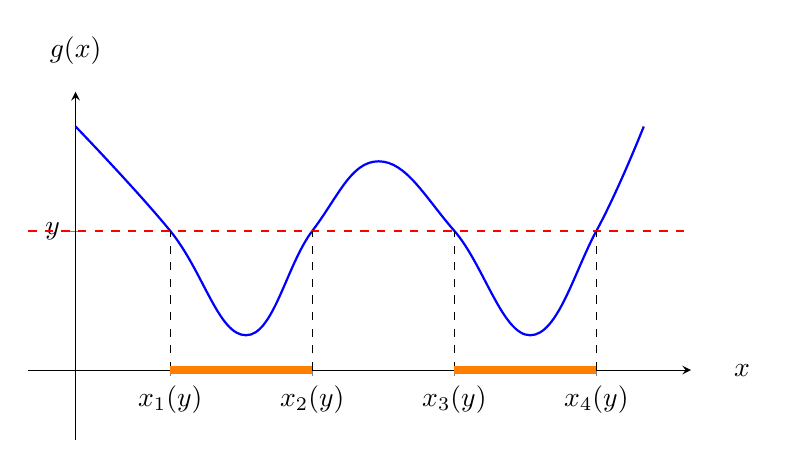
\begin{tikzpicture}
    \begin{axis}[
        width=10cm, height=6cm,
        axis lines=middle,
        xlabel={$x$}, ylabel={$g(x)$},
        xmin=-0.5, xmax=6.5,
        ymin=-1, ymax=4,
        xtick={1, 2.5, 4, 5.5},
        xticklabels={$x_1(y)$, $x_2(y)$, $x_3(y)$, $x_4(y)$},
        ytick={2},
        yticklabels={$y$},
        every axis x label/.style={at={(ticklabel* cs:1.05)}, anchor=west,},
        every axis y label/.style={at={(ticklabel* cs:1.05)}, anchor=south,},
    ]
        % Curva generica
        \addplot [thick, blue, smooth, tension=0.7] coordinates {
            (0, 3.5) (1, 2) (1.8, 0.5) (2.5, 2) (3.2, 3) (4, 2) (4.8, 0.5) (5.5, 2) (6, 3.5)
        };
        
        % Retta orizzontale y
        \addplot [dashed, red, thick] coordinates {(-0.5, 2) (6.5, 2)};
        
        % Linee verticali
        \draw[dashed] (axis cs:1,0) -- (axis cs:1,2);
        \draw[dashed] (axis cs:2.5,0) -- (axis cs:2.5,2);
        \draw[dashed] (axis cs:4,0) -- (axis cs:4,2);
        \draw[dashed] (axis cs:5.5,0) -- (axis cs:5.5,2);
        
        % Evidenziazione intervalli in cui la curva è sotto y
        \draw[line width=3pt, orange] (axis cs:1,0) -- (axis cs:2.5,0);
        \draw[line width=3pt, orange] (axis cs:4,0) -- (axis cs:5.5,0);
    \end{axis}
\end{tikzpicture}
\end{center}

Analizzando il grafico da sinistra a destra:
\begin{itemize}
    \item La funzione scende e interseca $x_1$ (derivata negativa: $g'(x_1) < 0$), la curva è sotto la retta $y$.
    \item La funzione risale e incontra $x_2$ ($g'(x_2) > 0$). Tra $x_1$ e $x_2$ la curva era sotto.
    \item Riscende e taglia in $x_3$ ($g'(x_3) < 0$).
    \item Risale e taglia in $x_4$ ($g'(x_4) > 0$), quindi tra $x_3$ e $x_4$ la curva era sotto $y$.
\end{itemize}

L'evento $Y \le y$ si verifica se la $X$ cade nel primo intervallo OPPURE nel secondo:
\begin{equation}
\mathbb{P}(Y \le y) = \mathbb{P}(x_1 \le X \le x_2) + \mathbb{P}(x_3 \le X \le x_4)
\end{equation}

Per quanto detto sulle CDF:
\begin{equation}
F_Y(y) = F_X(x_2) - F_X(x_1) + F_X(x_4) - F_X(x_3)
\end{equation}

Per trovare la PDF ci basta derivare:
\begin{equation}
f_Y(y) = f_X(x_2) \cdot x_2' - f_X(x_1) \cdot x_1' + f_X(x_4) \cdot x_4' - f_X(x_3) \cdot x_3'
\end{equation}

Per il teorema della funzione inversa $x'(y) = \frac{1}{g'(x)}$, quindi:
\begin{equation}
f_Y(y) = \frac{f_X(x_2)}{g'(x_2)} - \frac{f_X(x_1)}{g'(x_1)} + \frac{f_X(x_4)}{g'(x_4)} - \frac{f_X(x_3)}{g'(x_3)}
\end{equation}

Osservando i segni delle derivate (es. $g'(x_1)$ è negativa, quindi col segno meno davanti diventa positiva), si nota che i termini si sommano in valore assoluto. In generale la formula si compatta come:

\begin{equation}
\boxed{ f_Y(y) = \sum_{i=1}^{M(y)} \frac{f_X[x_i(y)]}{|g'[x_i(y)]|} }
\end{equation}


\subsection{Esercizio: Sia $g(x) = x^2$}

\subsubsection*{CASO 1: $X_1 \sim \mathcal{E}(\lambda)$}

La variabile esponenziale è definita solo per valori positivi o nulli. Il suo dominio ($\mathcal{X}_1$) è $[0, \infty[$. 
Vogliamo determinare $Y_1 = g(X_1) = X_1^2$.

\begin{center}
\begin{tikzpicture}
    \begin{axis}[
        width=6cm, height=4cm,
        axis lines=middle,
        xmin=-1, xmax=3,
        ymin=-1, ymax=5,
        xlabel={$x$}, ylabel={$y=x^2$},
        every axis x label/.style={at={(ticklabel* cs:1.05)}, anchor=west,},
        every axis y label/.style={at={(ticklabel* cs:1.05)}, anchor=south,}
    ]
        \addplot [thick, blue, domain=0:2.2] {x^2};
    \end{axis}
\end{tikzpicture}
\end{center}

Se disegni una parabola $y = x^2$ e consideri solo la parte di grafico che sta sulle $x$ positive, stai considerando una funzione strettamente crescente. Per quanto detto prima la funzione è invertibile (biettiva).
Siamo nel caso ``ideale''. Stiamo cercando $f_Y(y)$, tutto deve essere espresso in funzione di $y$.
Devo trovare $x$ che ha generato $y$, quindi ci serve l'inversa.

\begin{itemize}
    \item Risolviamo l'equazione: $x^2 = y \implies x(y) = \sqrt{y}$
    \item La derivata di $g(x) = x^2$ è $g'(x) = 2x$
\end{itemize}

Applicando la formula base per la trasformazione biettiva:
\begin{equation}
f_Y(y) = \frac{f_X(g^{-1}(y))}{(g)'(g^{-1}(y))} = \frac{\lambda e^{-\lambda x} \cdot u(x)}{2x} = \frac{\lambda e^{-\lambda \sqrt{y}}}{2\sqrt{y}} \cdot \overbrace{u(\sqrt{y})}^{u(y)}
\end{equation}


\subsubsection*{CASO 2: $X_2 \sim \mathcal{C}(0,1)$}

La variabile di Cauchy è definita su tutto l'asse reale ($\mathcal{X}_2 = \mathbb{R}$). 
Vogliamo determinare $Y_2 = g(X_2) = X_2^2$.

\begin{center}
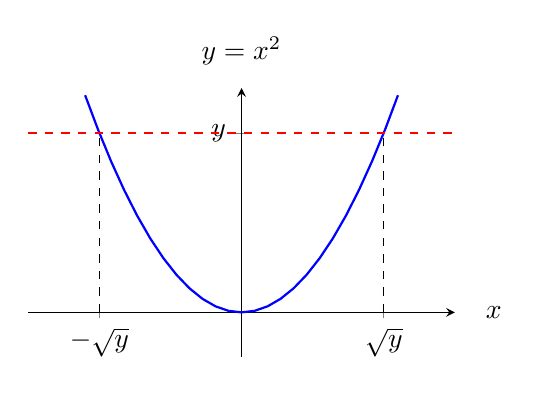
\begin{tikzpicture}
    \begin{axis}[
        width=7cm, height=5cm,
        axis lines=middle,
        xmin=-3, xmax=3,
        ymin=-1, ymax=5,
        xlabel={$x$}, ylabel={$y=x^2$},
        xtick={-2, 2},
        xticklabels={$-\sqrt{y}$, $\sqrt{y}$},
        ytick={4},
        yticklabels={$y$},
        every axis x label/.style={at={(ticklabel* cs:1.05)}, anchor=west,},
        every axis y label/.style={at={(ticklabel* cs:1.05)}, anchor=south,}
    ]
        \addplot [thick, blue, domain=-2.2:2.2] {x^2};
        \addplot [dashed, red, thick] coordinates {(-3, 4) (3, 4)};
        
        \draw[dashed] (axis cs:-2,0) -- (axis cs:-2,4);
        \draw[dashed] (axis cs:2,0) -- (axis cs:2,4);
    \end{axis}
\end{tikzpicture}
\end{center}

La funzione $y = x^2$ non è più invertibile su $\mathbb{R}$. La funzione scende, tocca lo $0$ e poi risale. $\forall y > 0$, la retta $y = y_0$ taglia la parabola in due punti.
Siamo nel caso ``reale''. $M(y) = 2$ intersezioni. Le due radici da cui posso arrivare a $y$ sono $x_1 = \sqrt{y}$ e $x_2 = -\sqrt{y}$.

Ricordiamo che la PDF di $X_2$ è $f_{X_2}(x) = \frac{1}{\pi(1+x^2)}$.
La derivata di $g(x) = x^2$ è $g'(x) = 2x \implies g'(x(y)) = \pm 2\sqrt{y}$.

Applicando la formula per la somma:
\begin{align}
f_Y(y) &= \sum_{i=1}^{M(y)} \frac{f_X[x_i(y)]}{|g'[x_i(y)]|} = \left[ \frac{f_X(\sqrt{y})}{2\sqrt{y}} + \frac{f_X(-\sqrt{y})}{2\sqrt{y}} \right] u(y) \nonumber \\
f_Y(y) &= \left( \frac{1}{2\pi\sqrt{y}} \cdot \frac{1}{1+y} + \frac{1}{2\pi\sqrt{y}} \cdot \frac{1}{1+y} \right) u(y) \nonumber \\
&= \frac{1}{\pi\sqrt{y}(1+y)} u(y)
\end{align}


\subsection{Qualche esempio - 2: Trasformazione Integrale di Probabilità}

Sia $X \sim f_X(x)$ una generica PDF. Usiamo come funzione di trasformazione la CDF della variabile stessa: $g(x) = F_X(x) = \mathbb{P}(X \le x)$.
Creiamo la nuova variabile $Y = F_X(X)$.

Siccome $Y$ è il risultato di una CDF, i suoi valori sono compresi tra $0$ e $1$. Quindi $\mathcal{Y} = [0, 1]$.
La CDF per definizione accumula probabilità, sale e resta costante, quindi è monotona crescente e invertibile.

\begin{itemize}
    \item Sia $y = F_X(x)$
    \item L'inversa è $x(y) = F_X^{-1}(y)$
    \item La derivata di $g(x) = F_X(x)$ è $g'(x) = f_X(x)$
\end{itemize}

Applichiamo la formula $f_Y(y) = \frac{f_X(x)}{|g'(x)|}$:
\begin{equation}
f_Y(y) = \frac{f_X[F_X^{-1}(y)]}{f_X[F_X^{-1}(y)]} = 1
\end{equation}

Per essere precisi sul dominio, possiamo scrivere:
\begin{equation}
f_Y(y) = \frac{f_X(F_X^{-1}(y))}{f_X(F_X^{-1}(y))} \cdot \Pi\left(y - \frac{1}{2}\right) \quad \text{dove} \quad \Pi(x) = 
\begin{cases} 
1 & |x| \le \frac{1}{2} \\ 
0 & |x| > \frac{1}{2} 
\end{cases}
\end{equation}

\begin{center}
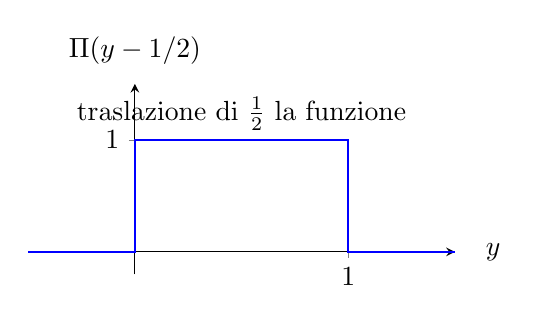
\begin{tikzpicture}
    \begin{axis}[
        width=7cm, height=4cm,
        axis lines=middle,
        xmin=-0.5, xmax=1.5,
        ymin=-0.2, ymax=1.5,
        xlabel={$y$}, ylabel={$\Pi(y - 1/2)$},
        xtick={0, 1},
        ytick={1},
        every axis x label/.style={at={(ticklabel* cs:1.05)}, anchor=west,},
        every axis y label/.style={at={(ticklabel* cs:1.05)}, anchor=south,}
    ]
        \addplot [thick, blue] coordinates {(-0.5,0) (0,0) (0,1) (1,1) (1,0) (1.5,0)};
        \node[anchor=south] at (axis cs: 0.5, 1) {traslazione di $\frac{1}{2}$ la funzione};
    \end{axis}
\end{tikzpicture}
\end{center}

Il rettangolo (la funzione rect $\Pi$) è un modo per dire che la funzione vale solo tra 0 e 1.
Osserviamo che tale $f_Y(y)$ coincide con la PDF della variabile uniforme $\mathcal{U}(0, 1)$.

\begin{quote}
\textbf{Conclusione fondamentale:} Se prendi una variabile aleatoria qualsiasi e la usi nella sua stessa CDF, il risultato è sempre una distribuzione uniforme tra 0 e 1. Questo ha delle notevoli conseguenze nelle procedure di simulazione dei sistemi numerici.
\end{quote}